\chapter{Supporting User Privacy Preferences in Digital Interactions}
\label{ch.privacy_pref}
%Alessandro
%%%%%%%%%%%%%%%%%%%%%%%%%%%%%%%%%%%%%%%%%%%%%%%%

\section{Introduzione}
Per la disponibilità dei servizi online si verifica la situazione in cui il server che fornisce il servizio e l'utente che lo richiede sono ignoti l'uno all'altro.
Di conseguenza sistemi di access control tradizionali non possono essere adottati in quanto non adatti a scenari open.

Soluzioni proposte sono basate su ABAC (Attribute-Based Access Control).
Policy che regolamentano l'accesso ai servizi definiscono condizioni che il client richiedente deve soddisfare per avere accesso.

Il server, a seguito di una richiesta di accesso risponde con le condizioni che il client deve soddisfare per essere autorizzato ad accedere al servizio.

$\\$
Per accedere il client rilascia \textbf{certificati digitali} come \textbf{credenziali} firmate da una \textbf{CA}.
L'adozione delle credenziali nell'Access Control ha diversi vantaggi:
\begin{itemize}
    \item Non serve $<$\textit{username,password}$>$ per ogni servizio.
    \item Offre migliore protezione dall'acquisizione impropria dei privilegi di accesso.
\end{itemize}

$\\$
L'uso di credenziali è stata approfonditamente studiata dal lato server con definizione di diversi \textit{policy languages}, \textit{policy engines} e strategie per la comunicazione delle consizioni di accesso.

Le soluzioni trovate, sebbene potenti ed espressive, non supportano completamente gli specifici criteri di protezione dei client.
Infatti i client necessitano di un sistema di preferenze che permetta di supportare una propria definizione di sensitivity/privacy per i propri dati.
Queste preferenze verranno poi usate nella situazione in cui più di un subset di credenziali soddisfano la Access Control Policy definita dal server.




Questo capitolo mostra una overview delle problematiche di privacy legate ai sistemi open, oltre che alcune soluzioni.
Le sezioni riportano invece:
\begin{itemize}
    \item Concetti Base e \textit{Desiderata}
    \item a 
    \item V
    \item c
    \item d
\end{itemize}


\section{Concetti Base e \textit{Desiderata}}

\subsection{Client Portfolio}

\begin{definition}[\textit{Client} Portfolio] $\\$
    Insieme delle informazioni che un cliente può fornire al server per avere accesso ad un servizio è racchiuso in un \textbf{Portfolio} contenente \begin{itemize}
        \item \textbf{Credenziali} firmate da third party.
        \item \textbf{Dichiarazioni} che comprendono proprietà non certificate dichiarate dall'utente.
    \end{itemize} 
\end{definition}

\subsubsection{Struttura Credenziale}
Ogni credenziale $c$ è composta da:
\begin{itemize}
    \item Identificatore univoco $id(c)$.
    \item Emittente $issuer(c)$.
    \item Un set di attributi $attributes(c)$.
    \item La tipologia della credenziale $type(c)$.
\end{itemize}


\subsubsection{Gerarchia Tipologie}
I tipi di credenziale sono organizzati tipicamente in una gerarchia radicata, dove i nodi intermedi sono astrazione delle specifiche credenziali presenti sulle foglie. Un esempio è in fig. \ref{fig:00_pref_cred_hierarchy}.

\begin{figure}[ht]
    \centering
    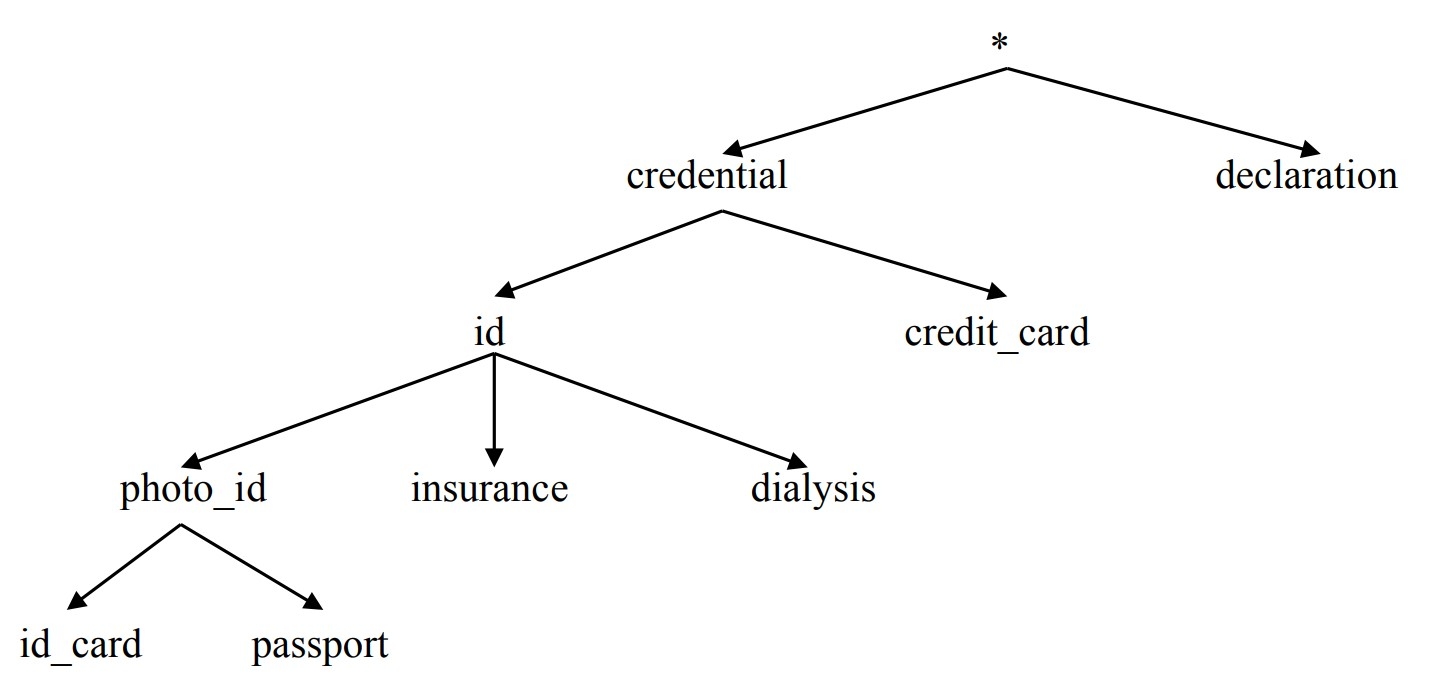
\includegraphics[width=0.8\textwidth]{paper_user-privacy-preferences/00_pref_credential_hierarchy.jpg}
    \caption{}
    \label{fig:00_pref_cred_hierarchy}
\end{figure}

La gerarchia è nota sia al client che al server. Il server tuttavia crea richieste di credential types in quanto non può conoscere le effettive credenziali possedute dal client\footnote{Inoltre client può avere più credenziali dello stesso tipo}.

\subsection{Atomicità Credenziali}
Le credenziali si distinguono in \textbf{atomiche} e \textbf{non-atomiche}.

$\\$
Le credenziali \textbf{atomiche} sono la tipologia più comune (vedi X.509) e possono essere rilasciato solo interamente.
Per questo anche attributi non richiesti vengono rivelati al server.

$\\$
Le credenziali \textbf{non-atomiche} permettono di limitare il rilascio di attributi rivelando selettivamente un subset degi attributi certificati dalla credenziale.

$\\$
Ovviamente le \textit{declaration} sono credenziali non-atomiche.


\subsubsection{Attributi}
Attributi nelle credenziali sono caratterizzati da:
\begin{itemize}
    \item Tipo
    \item Nome
    \item Valore
\end{itemize}
Essi possono essere \textit{credential-independent} e dipendere dal client ma non dalla credenziale, o \textit{credential-dependent} e dipendere da client e credenziale che la certifica.



\subsection{Policy di Disclosure}


